\documentclass[conference]{IEEEtran}

% ----------------------------
% Packages
% ----------------------------
\usepackage[utf8]{inputenc}
\usepackage{xfrac}
\usepackage{amsmath, amssymb, amsthm}
\usepackage{graphicx}
\usepackage[bookmarks=true,hidelinks]{hyperref}
\usepackage{cite}
\usepackage{booktabs}
\usepackage{multirow}
\usepackage{tikz}
\usepackage{etoolbox}
\usepackage{enumerate}
\usepackage[most]{tcolorbox}
\usepackage[font=small,labelfont=bf,labelsep=colon,justification=centering]{caption}
\captionsetup[table]{position=bottom} % put captions below tables
\tcbuselibrary{theorems}

\newtheorem{definition}{Definition}[section]

\tcolorboxenvironment{definition}{
  colback=blue!5!white,
  colframe=blue!30!black,
  boxrule=0.8pt,
  arc=2mm,
  left=1mm,
  right=1mm,
  top=1mm,
  bottom=1mm,
  enhanced,
  sharp corners,
  fonttitle=\bfseries,
  title style={font=\bfseries},
  before skip=0.6em, after skip=0.6em,
}

\newtheorem{proposition}{Proposition}[section]

\tcolorboxenvironment{proposition}{
  colback=green!5!white,
  colframe=green!30!black,
  boxrule=0.8pt,
  arc=2mm,
  left=1mm,
  right=1mm,
  top=1mm,
  bottom=1mm,
  enhanced,
  sharp corners,
  fonttitle=\bfseries,
  title style={font=\bfseries},
  before skip=0.6em, after skip=0.6em,
}

\tcolorboxenvironment{proof}{
    colback=red!5!white,
    colframe=red!30!black,
    boxrule=0.8pt,
    arc=2mm,
    left=1mm,
    right=1mm,
    top=1mm,
    bottom=1mm,
    enhanced,
    sharp corners,
    fonttitle=\bfseries,
    title style={font=\bfseries},
    before skip=0em, after skip=0.6em,
}

\newtheorem{theorem}{Theorem}[section]
\newtheorem{lemma}{Lemma}[section]

\tcolorboxenvironment{lemma}{
    colback=cyan!5!white,
    colframe=cyan!30!black,
    boxrule=0.8pt,
    arc=2mm,
    left=1mm,
    right=1mm,
    top=1mm,
    bottom=1mm,
    enhanced,
    sharp corners,
    fonttitle=\bfseries,
    title style={font=\bfseries},
    before skip=0.6em, after skip=0.6em,
}

\newtheorem{corollary}{Corollary}[section]

\newenvironment{note}{\par\color{teal}\begin{quote}\textbf{Note:}}{\end{quote}}

\tcbset{theorem style=plain}
\tcbset{coltitle=black, fonttitle=\bfseries}

% ----------------------------
% Title
% ----------------------------
\title{\huge Graph-Based Analysis of Solution Spaces in the Game \textit{Diplomatico}}

\author{
    \IEEEauthorblockN{Filippo Garagnani}
    \IEEEauthorblockA{
        Dipartimento di Ingegneria "Enzo Ferrari" \\
        Università degli Studi di Modena e Reggio Emilia \\
        \texttt{298707@studenti.unimore.it}
    }
}

\begin{document}
\maketitle

\begin{abstract}
The game of \textit{Diplomatico} (also known as 'The 100 Squares Puzzle' or 'Hopido' \cite{hopido}) has been studied during the last decades. 
The few results found are limited to determining whether the game is solvable or not for certain given constraints.
However, to the best of our knowledge, no one has ever tried to analyze different approaches to explore the solution space in its entirety.
In this work, we model the game as a graph where nodes represent squares and edges represent valid moves between these cells. 
We apply various graph analytics techniques to uncover structural properties of the solution space, identify key states, and explore potential strategies for solving the game.
\end{abstract}

% ----------------------------
% Sections
% ----------------------------

\section{Introduction}
The game of \textit{Diplomatico} is a combinatorial puzzle played on a rectangular grid. 
The objective is to fill the grid with consecutive numbers, subject to the following rules:
\begin{enumerate}
	\item The number $1$ may be placed on any available square.
	\item For $i > 1$, the number $i$ must be placed either at a distance of $3$ horizontally or vertically, or at a distance of $2$ diagonally from the square containing $i-1$.
	\item If no valid square is available for placing $i$, the game ends.
\end{enumerate}

An example of valid moves is shown in Figure~\ref{fig:example_moves}. 
Here, the number $2$ is placed diagonally with respect to $1$, while $3$ follows by a horizontal move from $2$.

\begin{figure}[ht]
	\centering
	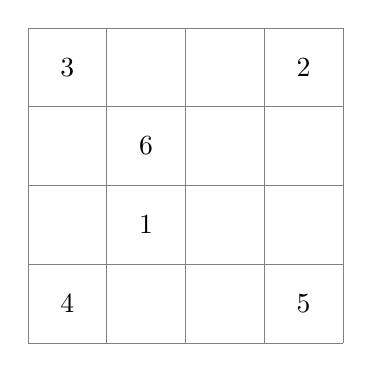
\begin{tikzpicture}
		\draw[step=1cm,gray,very thin] (0,0) grid (4,4);
		\node at (1.5,1.5) {$1$};
		\node at (3.5,3.5) {$2$};
		\node at (0.5,3.5) {$3$};
		\node at (0.5,0.5) {$4$};
		\node at (3.5,0.5) {$5$};
		\node at (1.5,2.5) {$6$};
	\end{tikzpicture}
	\caption{A $4 \times 4$ grid following the rules of \textit{Diplomatico}.}
	\label{fig:example_moves}
\end{figure}

Although the game is often introduced on square grids, this restriction is not essential: \textit{Diplomatico} can also be played on rectangular grids of arbitrary size, possibly with some cells blocked (i.e., unavailable for placement).

A few preliminary results are immediate. 
In particular, the game is unsolvable for square grids of size $4 \times 4$ or smaller, except for the trivial case of a $1 \times 1$ grid (see Figure~\ref{fig:trivial_case}).

\begin{figure}[ht]
	\centering
	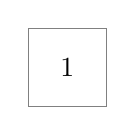
\begin{tikzpicture}
		\draw[step=1cm,gray,very thin] (0,0) grid (1,1);
		\node at (0.5,0.5) {$1$};
	\end{tikzpicture}
	\caption{The trivial case of a $1 \times 1$ grid.}
	\label{fig:trivial_case}
\end{figure}

The rules of the game admit a natural graph-theoretic formulation. 
Each cell of the grid is represented as a node, and a valid move (as defined above) corresponds to a directed edge between two nodes. 
Thus, constructing a valid play corresponds to finding a directed Hamiltonian path in this graph. 
Since determining whether a Hamiltonian path exists is an NP-complete problem~\cite{np}, the complexity of solving \textit{Diplomatico} grows rapidly with the grid size. 
This observation motivates the need for efficient heuristics and search strategies. 
Some classical approaches (such as Warnsdorff's Rule~\cite{warnsdorff}) will be revisited in this context, along with new strategies inspired by graph-theoretic centrality measures. 
In particular, we will investigate the relationship between different centrality indices (betweenness, closeness, degree, eigenvector) and the number of Hamiltonian paths available on a given board configuration. 
This correlation analysis provides insight into the structural properties of the game graph and their potential role in guiding play.

\section{Preliminaries}
The following definitions are used throughout this work. The main case being considered is the one in which the game grid is rectangular and doesn't have any cell blocked.

\begin{definition}{Board Graph}{}
\label{def:board_graph}

Given a board of size $n \times m$ (with $n, m \in \mathbb{N}$), the \textbf{Board Graph} of size $n \times m$ is an undirected graph $\mathfrak{G}_{n \times m} = (V, E)$, where:
$$
    V = \{v_{i,j},\;i = 1,\,\dots,\,n \land \, j = 1,\,\dots,\,m\}
$$
and where the following condition holds:
\begin{align*}
\forall e = \{v_{i,j},\;v_{k,\ell}\} \in E,\quad&(|i - k| = 3 \land j = \ell) \\
\lor\,& (|j - \ell| = 3 \land i = k) \\
\lor\,& (|i - k| = |j - \ell| = 2)
\end{align*}

\end{definition}

Of course, the node $v_{ij}$ will represent the square located at row $i$ and column $j$ of the original grid of the game. 
The condition required for the edge set $E$ ensures that only legal moves are present as undirected arcs in a Board Graph. The edges are undirected because, of course, the movement rules are perfectly simmetrical (i.e., being able to move from cell $A$ to cell $B$ means that it's also possible to move from cell $B$ to cell $A$).

\begin{definition}{Winning Path}{} \label{def:winning_path}
Given a Board Graph $\mathfrak{G}_{n \times m} = (V, E)$, a \textbf{Winning Path} is an Hamiltonian Path in $\mathfrak{G}_{n \times m}$.
Specifically, an Hamiltonian Path is a sequence of vertices $\mathfrak{h} = (v^1,\,v^2,\,\dots,\,v^{n \times m})$ such that:
$$
    \forall \ell = 1,\,\dots,\,k-1,\;\; \{v^\ell, v^{\ell+1}\} \in E
$$
and such that:
$$
    \forall v \in V,\;\; \exists!\, v^\ell \in \mathfrak{h} : v^\ell = v
$$
\end{definition}

An Hamiltonian Path is simply, as the Definition \ref{def:winning_path} gives, a path in the graph that visits every node exactly once.

\begin{definition}{Solvability}{}
\label{def:solvability}

Given a Board Graph $\mathfrak{G}_{n \times m}$, it is said to be \textbf{solvable} if:
\begin{align*}
    \exists &\mathfrak{h} = (v^1,\,v^2,\,\dots,\,v^{n \times m}) : \\
            &\mathfrak{h} \text{ is a Winning Path in } \mathfrak{G}_{n \times m}.
\end{align*}
\end{definition}

Definition \ref{def:solvability} simply states that a Board Graph is solvable if it contains at least one Hamiltonian Path; that is, if there is a way to start from a node (i.e., a cell in the game of \textit{Diplomatico}), and to be able to reach every other node - exactly once - by following the game rules. 

Simply from the Definitions \ref{def:board_graph}-\ref{def:solvability}, it is possible to prove the following Proposition.

\begin{figure}[ht]
	\centering
	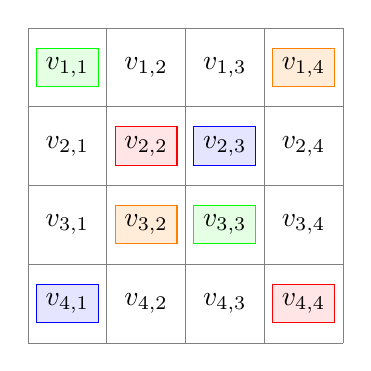
\begin{tikzpicture}
		\draw[step=1cm,gray,very thin] (0,0) grid (4,4);
		\foreach \x in {1,2,3,4} {
			\foreach \y in {1,2,3,4} {
				\ifnum\x=\y
				\pgfmathparse{mod(\x,2)==0}
				\ifnum\pgfmathresult=1
				\node[fill=red!10, draw=red] at (\x-0.5,4.5-\y) {$v_{\y,\x}$};
				\else
				\node[fill=green!10, draw=green] at (\x-0.5,4.5-\y) {$v_{\y,\x}$};
				\fi
				\else
				\pgfmathparse{\x+\y==5}
				\ifnum\pgfmathresult=1
				\pgfmathparse{mod(\x,2)==0}
				\ifnum\pgfmathresult=1
				\node[fill=orange!15, draw=orange] at (\x-0.5,4.5-\y) {$v_{\y,\x}$};
				\else
				\node[fill=blue!10, draw=blue] at (\x-0.5,4.5-\y) {$v_{\y,\x}$};
				\fi
				\else
				\node at (\x-0.5,4.5-\y) {$v_{\y,\x}$};
				\fi
				\fi
			}
		}
	\end{tikzpicture}
	\caption{The board representing the graph $\mathfrak{G}_{4 \times 4}$. In corresponding colors, the only possible edges from each central node.}
	\label{fig:dim_unsolvability_4x4}
\end{figure}

\begin{proposition}{Unsolvability of $\mathfrak{G}_{4 \times 4}$}{}
\label{prop:unsolvability_4x4}

The Board Graph $\mathfrak{G}_{4 \times 4}$ is unsolvable.
\end{proposition}
\begin{proof}
We can prove the unsolvability of $\mathfrak{G}_{4 \times 4}$ by contradiction. Assume that there exists a Winning Path $\mathfrak{h} = (v^1,\,v^2,\,\dots,\,v^{16})$ in $\mathfrak{G}_{4 \times 4}$. 

Since $\mathfrak{h}$ is a Hamiltonian Path, it must visit every node exactly once.
Consider the nodes in the center of the board - specifically, vertices $v_{2,2},\,v_{2,3},\,v_{3,2},\,v_{3,3}$ (see Figure \ref{fig:dim_unsolvability_4x4}).
Being $\mathfrak{G}_{4 \times 4}$ a Board Graph, the conditions for edges linking those vertices can be explicitly determined (focusing, for the time being, on $v_{2,2}$):
\begin{align*}
    &\forall e = \{v_{2,2},\;v_{i,j}\} \in E,\\
    &(|2 - i| = 3 \land 2 = j) \implies v_{i,j} \in \{v_{5,2},\,v_{-1,2}\}\\
    &(|2 - j| = 3 \land 2 = i) \implies v_{i,j} \in \{v_{2,5},\,v_{2,-1}\}\\
    &(|2 - i| = |2 - j| = 2) \implies v_{i,j} \in \{v_{0,0},\,v_{0,4},\,v_{4,0},\,v_{4,4}\}
\end{align*}
However, of the 'suggested' nodes above, only $v_{4,4}$ is actually present in $\mathfrak{G}_{4 \times 4}$ (the others are to consider 'out of bounds').
This means that the node $v_{2,2}$ can only be connected to $v_{4,4}$, implying that it must be either the first or the last node in the Winning Path $\mathfrak{h}$ (since it has degree $1$).
The same reasoning can be applied to the other three 'central' nodes; this means that four nodes must either be first or last in the path. This is not possible, hence the contradiction.

\end{proof}

The following Definition and Proposition will give a sense to the complexity of the game, and to the main focus of the work.

\begin{definition}{Numbers of Solutions}{}
\label{def:number_of_solutions}

Given a Board Graph $\mathfrak{G}_{n \times m}$, the \textbf{Number of Solutions} $\mathbf{N}(\mathfrak{G}_{n \times m})$ is defined as:
$$
    \mathbf{N}(\mathfrak{G}_{n \times m}) = |\{\mathfrak{h} : \mathfrak{h} \text{ is a Winning Path in } \mathfrak{G}_{n \times m}\}|
$$

\end{definition}

\begin{proposition}{Bounds on $\mathbf{N}(\mathfrak{G}_{n \times m})$}{}
\label{prop:bounds_number_of_solutions}

Given a Board Graph $\mathfrak{G}_{n \times m}$, with $n, m \ge 5$:
$$
    2^{(n - 4)(m - 4)/25} \le \mathbf{N}(\mathfrak{G}_{n \times m}) < 7^{nm - 1}
$$
\end{proposition}

The proof of Proposition \ref{prop:bounds_number_of_solutions} is given in Appendix \ref{appendix:proof_bound}.

The derived bounds demonstrate that the number of solutions increases exponentially with the board's size. This exponential growth renders exhaustive search methods infeasible for larger boards, emphasizing the necessity for more efficient algorithms and heuristics to navigate the solution space effectively. 
Furthermore, identifying even a single solution is a challenging task. The subsequent sections will delve into different search strategies and evaluate their performance.

\section{Implementation}									\label{sec:implementation}
\subsubsection{Finding solutions}
In order to efficiently analyze the solution space in the game of \textit{Diplomatico}, a few implementations have been developed.
Three of them were done in Neo4J \cite{neo4j}, leveraging its graph database capabilities to model the Board Graphs and perform various queries. To make the comparison valuable, another implementation in Python has been tested along the other.
Before any query is run, the Board Graph is generated and stored in the database offered by Neo4J through a simple script that simply requires the number of rows and of columns of the board.
Moreover, each query can be edited by command line arguments, by specifying - if needed - the start node of the path, the end node of the path and the total number of paths required.

The four main implementations of solution searching are briefly described below.

\paragraph{The \texttt{Raw} Implementation}
The \texttt{Raw} implementation is a straightforward query in Neo4J, which tries to expand from a starting node to find one or more Winning Paths.

\begin{tcolorbox}[colback=yellow!5!white, colframe=yellow!50!black]
\begin{verbatim}
MATCH p = (start:Node)
 -[:MOVE*{parameters["pathLength"]}]->
          (end:Node)
WHERE ALL(
    n IN nodes(p) WHERE 
    single(m IN nodes(p) WHERE m = n)
    )
RETURN p
\end{verbatim}
\end{tcolorbox}

The query above simply matches a path $p$ starting from any node labeled as \texttt{Node}, and tries to expand it by the number of edges specified in the parameter \texttt{pathLength} (which should be equal to $n \times m - 1$ for a board of size $n \times m$).
The \texttt{WHERE} clause ensures that the path is Hamiltonian, by checking that every node in the path appears once and exactly once.

The starting node can be specified by preappending a \texttt{MATCH (start:Node \{row: r, col: c\})} clause before the main \texttt{MATCH} clause, where \texttt{r} and \texttt{c} are the row and column of the desired starting node. The same applies to the end node.
Moreover, the query could be modified to return only a few solutions (by adding a \texttt{LIMIT} clause at the end of the query).
Thanks to the Python API of Neo4J, the element inside the \texttt{parameters} dictionary is modified at runtime.

\paragraph{The \texttt{Constructive} Implementation}
The \texttt{Raw} query, albeit simple, shows a few issues. The main problem being that it first finds all the possible paths of length $n \times m - 1$, and then filters out the non-Hamiltonian ones. This means that, for larger boards, the query will take a very long time to complete - if it completes at all.
In order to address this issue, a more 'constructive' approach has been implemented. The idea is to start from a node, and to try to expand the path step by step, ensuring each time that the Hamiltonian property is preserved.
The query is built in Python in the following way:
\begin{tcolorbox}[colback=yellow!5!white, colframe=yellow!50!black]
\begin{verbatim}
MATCH (n0:Node)-[:MOVE]->(n1:Node)
WHERE id(n1) NOT IN {id(n0)}
MATCH (n1)-[:MOVE]->(n2:Node)
WHERE id(n2) NOT IN {id(n0), id(n1)}
...
\end{verbatim}
\end{tcolorbox}

The query then contains every full path at the end, and these are guaranteed by construction to be Hamiltonian.
The starting and ending nodes can be specified in the same way as in the \texttt{Raw} implementation, as well as limiting to only a few solutions.

\paragraph{The \texttt{APOC} Implementation}
The \texttt{APOC} library \cite{apoc} for Neo4J contains the \texttt{apoc.path.expandConfig} procedure. By leveraging its parameters, it's possible to convert it into an Hamiltonian-finding algorithm.
\begin{tcolorbox}[colback=yellow!5!white, colframe=yellow!50!black]
\begin{verbatim}
MATCH (start:Node)
CALL apoc.path.expandConfig(
startNode, {
relationshipFilter: "MOVE>",
minLevel: {parameters["pathLength"]},
maxLevel: {parameters["pathLength"]},
uniqueness: "NODE_GLOBAL",
labelFilter: 'Node'
}
    ) YIELD path
\end{verbatim}
\end{tcolorbox}

If needed, the starting node can be specified in the same way as in the previous implementations; the ending node can be passed as an additional parameter to the APOC function itself, just like the number of paths to return.

\paragraph{The \texttt{Python} Implementation}
The last implementation is a pure Python one. It makes use of a backtracking algorithm to find one or more Winning Paths in a Board Graph.
The algorithm is implemented in a recursive way, and it can be summarized as follows:
\begin{tcolorbox}[colback=yellow!5!white, colframe=yellow!50!black]
\begin{verbatim}
find_path(current_path, board):
    if current_path covers all nodes:
        return current_path;
    for each move:
        add move to current_path;
        find_path(current_path, board);
        remove move from current_path;
\end{verbatim}
\end{tcolorbox}

Another known problem, similar to \textit{Diplomatico}, is the knight's tour problem.
A well known heuristics for that problem is the Warnsdorff's rule \cite{warnsdorff}: this says to first visit nodes with fewest moves available.
This heuristics has been implemented in the Python solution as well, and the effects of this rule over the speed of resolution has been analyzed in Section \ref{sec:results}.

\subsubsection{Centrality Measures}
The aim of this work also included the analysis of some graph-theoretic centrality measures to provide specific heuristics for solving a Board Graph. For analysis purposes, these can be directly computed inside a Neo4J server through the apposite \texttt{gds} library \cite{gds}. The centrality measures employed are listed below.

\paragraph{Degree Centrality} Given an undirected graph $G = (V, E)$, the \textbf{degree centrality} of a node $v \in V$ is exactly the number of edges this node has:
$$
	C_D(v) = |\{e \in E | v \in e\}|
$$
This value can be normalized by dividing each node's value by the maximum centrality found within the graph.

\paragraph{Betweeness Centrality}
Given a graph $G = (V, E)$, the \textbf{betweenness centrality} of a node $v \in V$ is defined as the number of shortest paths between pairs of nodes that pass through $v$. 
Formally, let $\sigma_{st}$ be the total number of shortest paths between nodes $s, t \in V$, and let $\sigma_{st}(v)$ be the number of those paths that pass through $v$. 
Then
$$
C_B(v) = \sum_{\substack{s, t \in V \\ s \neq v \neq t}} \frac{\sigma_{st}(v)}{\sigma_{st}}.
$$
Nodes with high betweenness act as bridges, controlling the flow of information between different regions of the graph.

\paragraph{Closeness Centrality} 
The \textbf{closeness centrality} of a node $v \in V$ measures how close $v$ is to all other nodes in the graph. 
It is defined as the reciprocal of the sum of the shortest-path distances $d(v,u)$ from $v$ to every other node $u \in V$: 
$$
C_C(v) = \frac{1}{\sum_{u \in V \setminus \{v\}} d(v, u)}.
$$
Nodes with high closeness centrality can reach other nodes quickly and are often well-positioned to spread information.

\paragraph{Eigenvector Centrality} 
The \textbf{eigenvector centrality} of a node $v \in V$ assigns relative scores to nodes such that connections to high-scoring nodes contribute more than connections to low-scoring ones. 
Formally, it is defined as the $v$-th component of the principal eigenvector of the adjacency matrix $A$ of the graph:
$$
C_E(v) = \frac{1}{\lambda} \sum_{u \in V} A_{vu} C_E(u),
$$
where $\lambda$ is the largest eigenvalue of $A$. 
This centrality highlights nodes that are influential not just by their degree, but by being connected to other important nodes.

\section{Results and Discussion}
\label{sec:results}

In this section, the results of the different approaches in finding Hamiltonian paths for the \textit{Diplomatico} graphs are analyzed, along with some improved versions enhanced by the results of the centrality measures.
The experiments were conducted on Neo4J version 2025.07.01, the APOC library version 2025.07.1core and the gds library version 2.20.0. The softwares were given maximum 16GB of RAM to execute the code.

\subsubsection{Searching the Solution Space}
The results shown in Table \ref{tab:onesol} have been obtained by running each query - or algorithm - $5$ times, and by averaging the time taken to complete the task.
The starting node and the ending node were not specified, and only one solution was required.

\begin{table}[ht]
\centering
\begin{tabular}{|c|c c c c |}
\hline
\textbf{Board Size} & \textbf{Raw} & \textbf{Constructive} & \textbf{APOC} & \textbf{Python} \\ \hline
\textbf{$4 \times 5$} & 0.4797s & 1.3337s & 0.1615s & \textbf{0.0085s}  \\ \hline
\textbf{$4 \times 6$} & $>$30s & 2.3749s & 0.2981s & \textbf{0.0180s} \\ \hline
\textbf{$4 \times 7$} & $>$30s & 4.4709s & 0.6444s & \textbf{0.1897s} \\ \hline
\textbf{$5 \times 5$} & $>$30s & 5.7675s & 0.7468s & \textbf{0.0040s} \\ \hline
\end{tabular}
\caption{Time results in finding only one solution for a certain board graph.}
\label{tab:onesol}
\end{table}

While, instead, the results shown in Tabel \ref{tab:onesolcon} have been obtained by running each query at the same conditions as above, but by also specifying the starting node as $v_{1,1}$ and the ending node as $v_{n,m}$ - the top-left and bottom-right corners of the board, respectively.

\begin{table}[ht]
\centering
\begin{tabular}{|c|c c c c |}
\hline
\textbf{Board Size} & \textbf{Raw} & \textbf{Constructive} & \textbf{APOC} & \textbf{Python} \\ \hline
\textbf{$4 \times 5$} & 0.7142s & 0.0417s & 0.0256s & \textbf{0.0032s}  \\ \hline
\textbf{$4 \times 6$} & $>$30s & 0.0659s & \textbf{0.0250s} & 0.0514s \\ \hline
\textbf{$4 \times 7$} & $>$30s & 3.2629s & \textbf{0.5479s} & 0.5982s \\ \hline
\textbf{$5 \times 5$} & $>$30s & 0.6837s & 0.4557s & \textbf{0.0147s} \\ \hline
\end{tabular}
\caption{Time results in finding only one solution, with constraints on the starting and ending nodes.}
\label{tab:onesolcon}
\end{table}

In Table \ref{tab:solscon}, instead, not only the starting and ending nodes were specified, but also every solution was required.

\begin{table}[ht]
\centering
\begin{tabular}{|c|c c c c |}
\hline
\textbf{Board Size} & \textbf{Raw} & \textbf{Constructive} & \textbf{APOC} & \textbf{Python} \\ \hline
\textbf{$4 \times 5$} & 1.1492s & 0.0331s & 0.0143s & \textbf{0.0034s} \\ \hline
\textbf{$4 \times 6$} & $>$30s & 0.6907s & \textbf{0.0307s} & 0.0503s \\ \hline
\textbf{$4 \times 7$} & $>$30s & 16.6208s & \textbf{0.6338s} & 0.6547s \\ \hline
\textbf{$5 \times 5$} & $>$30s & 3.1501s & 2.9022s & \textbf{0.4530s} \\ \hline
\end{tabular}
\caption{Time results in finding every solution, with constraints on the starting and ending nodes.}
\label{tab:solscon}
\end{table}

As it can be easily seen, the two most competitive implementations are the \texttt{APOC} one and the pure \texttt{Python} one.
In order to compare them, a few more tests have been conducted on larger boards - excluding the too slow \texttt{Raw} and \texttt{Constructive} implementations.
More specifically, each of the time results shown in Table \ref{tab:onesolL} has been obtained as a mean over $20$ runs; only one solution was required and no starting and ending node were specified.

\begin{table}[ht]
\centering
\begin{tabular}{|c|c c|}
\hline
\textbf{Board Size} & \textbf{APOC} & \textbf{Python} \\ \hline
\textbf{$5 \times 6$} & \textbf{0.0578s} & 0.4754s \\ \hline
\textbf{$4 \times 8$} & \textbf{3.9755s} & 6.3072s \\ \hline
\textbf{$5 \times 7$} & 0.1442s & \textbf{0.0007s} \\ \hline
\textbf{$6 \times 6$} & \textbf{0.2700s} & 0.5473s \\ \hline
\end{tabular}
\caption{Time results in finding only one solution for larger boards.}
\label{tab:onesolL}
\end{table}

As expected, as the board size increases, the time taken to find a solution has an exponential growth.
Curiously enough, it seems that - in general - solutions are easier to be find for more 'regular' board sizes, rather than very rectangular ones. Solutions also seem easier to find if the starting and ending node are specified - probably because this reduces the overall search space.
This could be due to the fact that, in more rectangular boards, there are less possible moves available from each node - hence, the search space is smaller.
Overall, the \texttt{APOC} implementation seems to be more stable in terms of time taken for runs, while the \texttt{Python} one starts going slower as the complexity rises.
The board $5 \times 7$ is solved very fast - probably due Warnsdorff's heuristics working accurately well in this particular case.

In Table \ref{tab:warn}, it has been compared the usage of the Warnsdorff's rule with a random choice for the nodes; the results have been obtained by averaging over $10$ runs of the algorithms. Except a few cases, as a rule of thumb, it could be said that employing Warnsdorff's rule for choosing the next node is an efficient strategy, improving by a bit the results in time complexity.

\begin{table}[ht]
	\setlength{\tabcolsep}{3pt}
	\centering
	\begin{tabular}{|c|c|c|c|c|c|c|c|}
		\hline
		 $4 \times 5$ & $4 \times 6$ & $4 \times 7$ & $5 \times 5$ & $5 \times 6$ & $4 \times 8$ & $5 \times 7$ & $6 \times 6$ \\ \hline
		 \scriptsize 0.0085s & \scriptsize \textbf{0.0180s} & \scriptsize\textbf{ 0.1897s} & \scriptsize \textbf{0.0040s} & \scriptsize 0.4754s & \scriptsize 6.3072s & \scriptsize \textbf{0.0007s} & \scriptsize \textbf{0.5473s} \\
		 \scriptsize  \textbf{0.0055s} & \scriptsize 0.0241s & \scriptsize 0.2776s & \scriptsize 0.0330s & \scriptsize \textbf{0.0462s} & \scriptsize \textbf{4.5177s} & \scriptsize $>$30s & \scriptsize 0.8116s \\ \hline
	\end{tabular}
	\caption{Comparison between employing Warnsdorff's rule (first row) or random nodes (second row).}
	\label{tab:warn}
\end{table}

Table \ref{tab:sols} shows a collection of the number of solutions for boards that have been completely explored.

\begin{table}[ht]
	\centering
	\begin{tabular}{|c|c|}
		\hline
		\textbf{Board Size} & \textbf{N° of Solutions} \\ \hline
		\textbf{$4 \times 5$} & 144	\\ \hline
		\textbf{$4 \times 6$} & 128	\\ \hline
		\textbf{$4 \times 7$} & 72  \\ \hline
		\textbf{$5 \times 5$} & 12400 \\ \hline 
	\end{tabular}
	\caption{Number of solutions for each board graph thouroghly analyzed.}
	\label{tab:sols}
\end{table}

\subsubsection{Starting Nodes}
The usage of centrality measures, as it will be seen, can be exploited to see how it relates to starting nodes. More specifically, it has been examined the relationships between the number of paths starting from a certain node $v_{i, j}$ and its centrality measures. In order to do so, Pearson's correlation has been analyzed - to find trends between these two variables. In order to make the analysis statistically significant, the relative \textit{p}-values are also analyzed to understand the likelihood of the findings. The results of the experiments can be found on Table \ref{tab:correlations}.

\begin{table}[ht]
	\centering
	\setlength{\tabcolsep}{4pt}
	\begin{tabular}{|llcccc|}
		\toprule
		\multirow{2}{*}{Board} & \multirow{2}{*}{Metric} & \multicolumn{4}{c}{Centrality Measure} \\
		\cmidrule(lr){3-6}
		& & Betweenness & Closeness & Degree & Eigenvector \\
		\midrule
		\multirow{2}{*}{$4 \times 5$} 
		& Correlation & \textbf{-0.8228}*** & -0.5899** & -0.7845*** & -0.1728 \\
		& $p$-value   & 0.0000 & 0.0062 & 0.0000 & 0.4664 \\
		\midrule
		\multirow{2}{*}{$4 \times 6$} 
		& Correlation & \textbf{-0.7744}*** & -0.6316*** & -0.7197*** & -0.5179** \\
		& $p$-value   & 0.0000 & 0.0009 & 0.0001 & 0.0095 \\
		\midrule
		\multirow{2}{*}{$5 \times 5$} 
		& Correlation & \textbf{-0.6820}*** & -0.2543 & -0.4037* & -0.1460 \\
		& $p$-value   & 0.0002 & 0.2199 & 0.0454 & 0.4861 \\
		\midrule
		\multirow{2}{*}{$4 \times 7$} 
		& Correlation & \textbf{-0.9098}*** & -0.8204*** & -0.8596*** & -0.5842** \\
		& $p$-value   & 0.0000 & 0.0000 & 0.0000 & 0.0011 \\
		\bottomrule
	\end{tabular}
	\caption{Correlation coefficients ($r$) and $p$-values between Hamiltonian paths and centrality measures across different board sizes.}
	\label{tab:correlations}
\end{table}

First of all, to comment these results, it can be easily seen that most of them - except a few - can be declared conclusive, thanks to the very low $p$-values.
Then, these results may seem counter-intuitive at first: they indicate that the higher the centrality values of a certain node, the lesser the number of Winning Paths will span starting from it. This, however, may be justified by the fact that starting from a more central node - for the beetweness centrality, a \textit{bottleneck} - may occlude more paths rather than starting from a more unreachable node.

\section{Conclusion and Future Work}
This work has presented a comprehensive graph-based analysis of the solution space in the game of \textit{Diplomatico}. By modeling the puzzle as a Board Graph and leveraging both Neo4J and Python implementations, we have demonstrated the exponential complexity inherent in enumerating Hamiltonian paths and provided empirical benchmarks for several search strategies. The results highlight the effectiveness of advanced graph database procedures (such as APOC) and heuristic-driven algorithms (notably Warnsdorff's rule) in efficiently navigating large solution spaces. 

Key findings include the derivation of theoretical bounds on the number of solutions, the identification of structural properties that impact solvability, and the comparative performance of different computational approaches. The experiments confirm that exhaustive search quickly becomes infeasible as board size increases, underscoring the need for scalable heuristics and optimized queries.

Future work may focus on extending these methods to boards with blocked cells, exploring parallelization strategies, and integrating machine learning techniques to predict solvability or guide search. Additionally, further theoretical investigation into tighter bounds and the combinatorial structure of solution spaces could yield deeper insights. The approaches and tools developed here provide just a solid foundation for still unexplored game of Diplomatico.

% ----------------------------
% References
% ----------------------------
\bibliographystyle{IEEEtran}
\bibliography{references}

\newpage
% IEEEtran prefers \appendices to format appendix headings correctly
\appendices
\section{Over the Bounds of the Number of Solutions} 	\label{appendix:proof_bound}
Here is the detailed proof of the lower bound referenced in the main text, specifically for Proposition \ref{prop:bounds_number_of_solutions}.
The first part - the upper bound - of the proof can be easily given, while a set of intermediate results are later needed for the second part of it - the lower bound.
\vspace{0.6em}
\begin{proof}
	\textbf{Upper Bound.} 
	Any winning path $\mathfrak{h}$ must pass from a 'corner' node (i.e., $v_{1,1},\,v_{1,m},\,v_{n,1},\,v_{n,m}$). By evaluating the possibilities, it can be easily determined that only three edges are connected to any corner node.
	\begin{align*}
		&\forall e = \{v_{1,1},\;v_{i,j}\} \in E, \\
		&(|1 - i| = 3 \land 1 = j) \implies v_{i,j} \in \{v_{4,1},\,v_{-2,1}\} \\
		&(|1 - j| = 3 \land 1 = i) \implies v_{i,j} \in \{v_{1,4},\,v_{1,-2}\} \\
		&(|1 - i| = |1 - j| = 2) \implies \\
		&\quad\quad v_{i,j} \in \{v_{3,3},\,v_{3,-1},\,v_{-1,3},\,v_{-1,-1}\}
	\end{align*}
	In this specific case, the only possible adjacent nodes are $v_{4,1},\,v_{1,4},\,v_{3,3}$. The same reasoning applies to the other corner nodes.
	
	Moreover, the start node - in the general scenario - will have at most $8$ edges connected to it (assuming, from the previous verification, that each node is valid). Every other node, however, will have at most $7$: surely, the edge chosen to reach it should not be considered, otherwise we would obtain a path that couldn't be Hamiltonian - reaching an already visited node.
	This means that, combinatorially speaking:
	$$
	\mathbf{N}(\mathfrak{G}_{n \times m}) \leq 8 \cdot 3^4 \cdot 7^{nm - 5} < 7^{nm - 1}
	$$
\end{proof}

To reach the second part of the proof, some handful lemmas are presented.

\begin{lemma} \label{lem:two_boards_horizontal}
    For any Board Graph $\mathfrak{G}_{n \times m}$ with $9 \ge n, m \ge 5$, there exist at least $2$ distinct Winning Path $\mathfrak{h}$ such that:
    $$
        \mathfrak{h}_1 = v_{3,\,1} \land \mathfrak{h}_{nm} = v_{3,\,m-2} 
    $$
\end{lemma}

The Lemma \ref{lem:two_boards_horizontal} can be proved, to the best of my knowledge, only by enumerating all the possible couples $(n,\,m)$ - with, without loss of generality, $n \ge m$, otherwise the indeces of the nodes could be easily swapped -
and by explicitly finding the $2$ distinct Winning Paths for each of them.
What the Lemma states is that there is a guarantee of $2$ different solutions which 'start' from the border node $v_{n-2,\,1}$ and that end with the node displaced by $2$ both horizontally and vertically from the outer edges.
This constraint guarantees the possibility to create a tilization of the board for every $n, m \ge 5$ - hence, guaranteeing a lower bound.

\begin{lemma} \label{lem:tiling}
    Given the Board Graph $\mathfrak{G}_{(n+k) \times m}$ with $9 \ge n, m, k \ge 5$, then $\mathfrak{G}_{(n + k) \times m}$ is solvable.
\end{lemma}
\begin{figure}[ht]
	\centering
	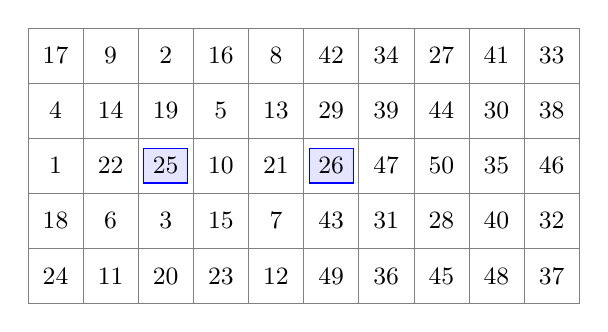
\begin{tikzpicture}[scale=0.7, every node/.style={font=\small}]
		\draw[step=1cm,gray,very thin] (0,0) grid (10,5);
		
		\node at (0.5,4.5) {17};
		\node at (1.5,4.5) {9};
		\node at (2.5,4.5) {2};
		\node at (3.5,4.5) {16};
		\node at (4.5,4.5) {8};
		
		\node at (0.5,3.5) {4};
		\node at (1.5,3.5) {14};
		\node at (2.5,3.5) {19};
		\node at (3.5,3.5) {5};
		\node at (4.5,3.5) {13};
		
		\node at (0.5,2.5) {1};
		\node at (1.5,2.5) {22};
		\node[fill=blue!10, draw=blue] at (2.5,2.5) {25};
		\node at (3.5,2.5) {10};
		\node at (4.5,2.5) {21};
		
		\node at (0.5,1.5) {18};
		\node at (1.5,1.5) {6};
		\node at (2.5,1.5) {3};
		\node at (3.5,1.5) {15};
		\node at (4.5,1.5) {7};
		
		\node at (0.5,0.5) {24};
		\node at (1.5,0.5) {11};
		\node at (2.5,0.5) {20};
		\node at (3.5,0.5) {23};
		\node at (4.5,0.5) {12};
		
		% Right half 
		\node at (5.5,4.5) {42};
		\node at (6.5,4.5) {34};
		\node at (7.5,4.5) {27};
		\node at (8.5,4.5) {41};
		\node at (9.5,4.5) {33};
		
		\node at (5.5,3.5) {29};
		\node at (6.5,3.5) {39};
		\node at (7.5,3.5) {44};
		\node at (8.5,3.5) {30};
		\node at (9.5,3.5) {38};
		
		\node[fill=blue!10, draw=blue] at (5.5,2.5) {26};
		\node at (6.5,2.5) {47};
		\node at (7.5,2.5) {50};
		\node at (8.5,2.5) {35};
		\node at (9.5,2.5) {46};
		
		\node at (5.5,1.5) {43};
		\node at (6.5,1.5) {31};
		\node at (7.5,1.5) {28};
		\node at (8.5,1.5) {40};
		\node at (9.5,1.5) {32};
		
		\node at (5.5,0.5) {49};
		\node at (6.5,0.5) {36};
		\node at (7.5,0.5) {45};
		\node at (8.5,0.5) {48};
		\node at (9.5,0.5) {37};
		
	\end{tikzpicture}
\caption{A $5 \times 10$ grid solved by tiling. The two halves have the same path connecting $v_{1,3}$ to $v_{3,3}$. In blue, the 'link' between two otherwise disjoint paths.}
\label{fig:tiling_example}
\end{figure}
	
\begin{proof}
    Consider the two Board Graphs $\mathfrak{G}_{n \times m}$ and $\mathfrak{G}_{k \times m}$.
    By Lemma \ref{lem:two_boards_horizontal}, both of them are solvable - since $9 \ge n, m, k \ge 5$.
    Let $\mathfrak{h}^1$ be one of the Winning Paths in $\mathfrak{G}_{n \times m}$ guaranteed to exists;
        and let $\mathfrak{h}^2$ be one of the Winning Paths in $\mathfrak{G}_{n \times k}$ guaranteed to exists.
    Defining $\hat{\mathfrak{h}}^2$ in the following way:
    $$
        \hat{\mathfrak{h}}^2 = (v_{i, j + m} : v_{i,j} \in \mathfrak{h}^2)
    $$
    So: the new defined path $\hat{\mathfrak{h}}^2$ is simply the path $\mathfrak{h}^2$ 'shifted' horizontally by $m$ columns.
        It can be proven that the following $\mathfrak{h}^3$ is indeed a Winning Path:
    $$
        \mathfrak{h}^3 = (\mathfrak{h}^1,\,\hat{\mathfrak{h}}^2)
    $$
    First of all, the two paths $\mathfrak{h}^1$ and $\hat{\mathfrak{h}}^2$ are disjoint, since they refer to different nodes of the graph; moreover, they completely 'touch' each node of the partitions, being Winning Paths.
    The only thing left to prove is that the last node of $\mathfrak{h}^1$ is connected to the first node of $\hat{\mathfrak{h}}^2$.
    By Lemma \ref{lem:two_boards_horizontal}, the last node of $\mathfrak{h}^1$ is $v_{3,\,m-2}$; while the first node of $\hat{\mathfrak{h}}^2$ is $v_{3,\,m+1}$.
    It can be easily verified that:
    $$
        (|m+1 - m-2| = 3 \land 3 = 3)
    $$
    hence, the edge $\{v_{3,\,m-2},\,v_{3,\,m+1}\}$ exists, giving a complete solution for the Board Graph $\mathfrak{G}_{(n + k) \times m}$.
\end{proof}

The result exposed in the Lemma \ref{lem:tiling} is graphically represented in Figure \ref{fig:tiling_example}.
It's to note that the above Lemma \ref{lem:tiling} can be easily adapted to increasing values of columns for Board Graphs.

The following Lemmas, instead, focus on stacking Board Graphs vertically.

\begin{lemma} \label{lem:two_boards_vertical}
    For any Board Graph $\mathfrak{G}_{n \times m}$ with $9 \ge n, m \ge 5$, there exist at least $2$ distinct Winning Path $\mathfrak{h}$ such that:
    $$
        \mathfrak{h}_1 = v_{3,\,1} \land \mathfrak{h}_{nm} = v_{n,\,m} 
    $$
\end{lemma}

Once again, a proof of the Lemma would require an enumeration of all the possible couples $(n,\,m)$, and their respective solved distinct Hamiltonian.
\begin{lemma} \label{lem:tiling_vertical}
    Given the Board Graph $\mathfrak{G}_{n \times (m + k)}$ with $9 \ge n, m, k \ge 5$, then $\mathfrak{G}_{n \times (m + k)}$ is solvable.
\end{lemma}
\begin{proof}
    Consider the two Board Graphs $\mathfrak{G}_{n \times m}$ and $\mathfrak{G}_{n \times k}$.
    Without loss of generality, assume $m \ge k$. Then, by knowing Lemma \ref{lem:two_boards_vertical}, both of them are solvable - since $9 \ge n, m, k \ge 5$.
    Let $\mathfrak{h}^1$ be one of the Winning Paths in $\mathfrak{G}_{n \times m}$ guaranteed to exist;
        and let $\mathfrak{h}^2$ be one of the Winning Paths in $\mathfrak{G}_{n \times k}$ guaranteed to exist, either by Lemma \ref{lem:two_boards_horizontal} or by Lemma \ref{lem:two_boards_vertical}.
    Then, define $\hat{\mathfrak{h}}^2$ in the following way:
    $$
        \hat{\mathfrak{h}}^2 = (v_{i + n, m - j + 1} : v_{i,j} \in \mathfrak{h}^2)
    $$
    This path $\hat{\mathfrak{h}}^2$ is simply the path $\mathfrak{h}^2$ swapped over the columns and 'shifted' vertically by $n$ rows.
        It can be proven that the following $\mathfrak{h}^3$ is indeed a Winning Path:
    $$
        \mathfrak{h}^3 = (\mathfrak{h}^1,\,\hat{\mathfrak{h}}^2)
    $$
    First of all, the two paths $\mathfrak{h}^1$ and $\hat{\mathfrak{h}}^2$ are disjoint, since they refer to different nodes of the graph; moreover, they completely 'touch' each node of the partitions, being Winning Paths.
    The only thing left to prove is that the last node of $\mathfrak{h}^1$ is connected to the first node of $\hat{\mathfrak{h}}^2$.
    By Lemma \ref{lem:two_boards_vertical}, the last node of $\mathfrak{h}^1$ is $v_{n,m}$ while the first node of $\hat{\mathfrak{h}}^2$ is $v_{n+3,\,m}$.
    It can be easily verified that:
    $$
        (|n+3 - n| = 3 \land m = m)
    $$
    Hence, the edge $\{v_{n,m},\,v_{n+3,\,m}\}$ exists, giving a complete solution for the Board Graph $\mathfrak{G}_{n \times (m + k)}$.
\end{proof}

\begin{figure}[ht]
\centering
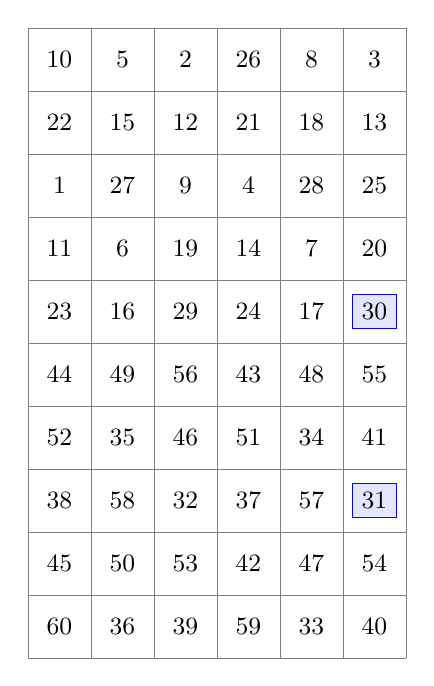
\begin{tikzpicture}[scale=0.8, every node/.style={font=\small}]
  \draw[step=1cm,gray,very thin] (0,0) grid (6,10);

  \node at (0.5,9.5) {10};
  \node at (1.5,9.5) {5};
  \node at (2.5,9.5) {2};
  \node at (3.5,9.5) {26};
  \node at (4.5,9.5) {8};
  \node at (5.5,9.5) {3};

  \node at (0.5,8.5) {22};
  \node at (1.5,8.5) {15};
  \node at (2.5,8.5) {12};
  \node at (3.5,8.5) {21};
  \node at (4.5,8.5) {18};
  \node at (5.5,8.5) {13};

  \node at (0.5,7.5) {1};
  \node at (1.5,7.5) {27};
  \node at (2.5,7.5) {9};
  \node at (3.5,7.5) {4};
  \node at (4.5,7.5) {28};
  \node at (5.5,7.5) {25};

  \node at (0.5,6.5) {11};
  \node at (1.5,6.5) {6};
  \node at (2.5,6.5) {19};
  \node at (3.5,6.5) {14};
  \node at (4.5,6.5) {7};
  \node at (5.5,6.5) {20};

  \node at (0.5,5.5) {23};
  \node at (1.5,5.5) {16};
  \node at (2.5,5.5) {29};
  \node at (3.5,5.5) {24};
  \node at (4.5,5.5) {17};
  \node[fill=blue!10, draw=blue] at (5.5,5.5) {30};

    \node at (0.5,4.5) {44};
    \node at (1.5,4.5) {49};
    \node at (2.5,4.5) {56};
    \node at (3.5,4.5) {43};
    \node at (4.5,4.5) {48};
    \node at (5.5,4.5) {55};

    \node at (0.5,3.5) {52};
    \node at (1.5,3.5) {35};
    \node at (2.5,3.5) {46};
    \node at (3.5,3.5) {51};
    \node at (4.5,3.5) {34};
    \node at (5.5,3.5) {41};

    \node at (0.5,2.5) {38};
    \node at (1.5,2.5) {58};
    \node at (2.5,2.5) {32};
    \node at (3.5,2.5) {37};
    \node at (4.5,2.5) {57};
    \node[fill=blue!10, draw=blue] at (5.5,2.5) {31};

    \node at (0.5,1.5) {45};
    \node at (1.5,1.5) {50};
    \node at (2.5,1.5) {53};
    \node at (3.5,1.5) {42};
    \node at (4.5,1.5) {47};
    \node at (5.5,1.5) {54};

    \node at (0.5,0.5) {60};
    \node at (1.5,0.5) {36};
    \node at (2.5,0.5) {39};
    \node at (3.5,0.5) {59};
    \node at (4.5,0.5) {33};
    \node at (5.5,0.5) {40};
\end{tikzpicture}
\caption{A $5 \times 6$ grid solved by tiling. The two halves have the same path, albeit rotated over the columns, connecting $v_{3,1}$ to $v_{5,6}$ and then $v_{8,6}$ and $v_{10,1}$. In blue, the 'link' between two otherwise disjoint paths.}
\label{fig:tiling_example_rectangular}
\end{figure}

\vspace{0.6em}
\begin{proof}
    \textbf{Lower Bound}. We will show that for any $n, m \ge 5$:
    $$
        \mathbf{N}(\mathfrak{G}_{n \times m}) \ge 2^{(n - 4)(m - 4)/25}
    $$
    To establish this, we can use a combinatorial argument based on the structure of the board graph.
    More specifically, given a generic Board Graph $\mathfrak{G}_{n \times m}$, we can partition it into smaller sub-graphs of size $5 \times 5$ plus - in case of $n,m$ not divisible by $5$ - some additional sub-graphs of size $k_i \times \ell_i$, with $9 \ge k_i, \ell_i \ge 5$.
    Thanks to Lemma \ref{lem:tiling} and Lemma \ref{lem:tiling_vertical}, we know that all these sub-graphs are solvable, and particularly that the whole Board Graph $\mathfrak{G}_{n \times m}$ is also solvable, by tiling the sub-graphs accordingly.
    
    The total number of sub-graphs in which to partition the original Board Graph is $\lfloor\dfrac{n}{5}\rfloor \cdot \lfloor\dfrac{m}{5}\rfloor$.
    This can be proven by simply considering that each sub-graph has a size of $5 \times 5$; hence, the number of sub-graphs that can fit in the original Board Graph is simply the integer division of the dimensions of the original graph by $5$.
    Each of these sub-graphs has at least $2$ distinct Winning Paths, as guaranteed by Lemma \ref{lem:two_boards_horizontal} and Lemma \ref{lem:two_boards_vertical}.
    This means that, combinatorially speaking, the total number of distinct Winning Paths in the original Board Graph is at least:
    $$
        \mathbf{N}(\mathfrak{G}_{n \times m}) \ge 2^{\lfloor n/5 \rfloor \cdot \lfloor m/5 \rfloor}
    $$
    In order to show the original, exponential in $n,m$, bound, it's only necessary to consider that:
    $$
        \lfloor n/5 \rfloor \ge (n - 4)/5
    $$
    This is because, in the worst case scenario, $n = 5 \times k + 4$; hence, $\lfloor n/5 \rfloor = k$ and $(n - 4)/5 = k$.
    The same reasoning applies to $m$; hence, the original bound is proven.
\end{proof}

\newpage
\section{Over the Creation of a Board Graph in Neo4J}		\label{appendix:neo4j}

In order to provide a common ground for retrieving a solution in Neo4J \cite{neo4j} (see Section \ref{sec:implementation}), a variable-dependent query was designed to create a Board Graph of desired size. The structure of the graph is organized in the following way:
\begin{itemize}
	\item Each node is created with the label \texttt{Node}, and has - as properties - \textit{row} and \textit{col}, respectively the indeces of row and of column in the original board-like structure.
	\item Each link between two nodes (present only if a legal move allows the movement between those two nodes) is created, with label \texttt{MOVE}.
\end{itemize}
The Python function implementing the creation of this query is described in the current Appendix in pseudocode.

\begin{tcolorbox}[colback=yellow!5!white, colframe=yellow!50!black]
\begin{verbatim}
create_graph_query(rows, cols):
	for i = 0, ..., rows - 1:
		for j = 0, ..., cols - 1:
			query += create_query(i, j)
\end{verbatim}
\end{tcolorbox}

This snippet regulates the creation of all the necessary nodes, each with its own specific properties. The code loops through all the possible row indices (from $0$ to the input parameter $\texttt{rows} - 1$) and through all the possible column indices. For every possible pair of row and column indices, then, it stores a line created by the method \texttt{create\_query(i, j)}. This returns the following query:
\begin{center}
	\texttt{"CREATE (n\_i\_j:Node \{row: i, col: j\})$\backslash$n"}
\end{center}
of course, substituting the two parameters $i,\,j$ with the passed values. For instance, for the node at position $(2, 3)$, the line will ask to create a node with label \texttt{Node}, called \texttt{n\_1\_2}, and with properties \texttt{row=}$1$ and \texttt{col=}$2$ (because values start from $0$).

\end{document}
